% =====================================================================
%  Data Mining · SGH · SMMD-ADA   —   Block 1 slide deck
%  Template: Frankfurt + seahorse + miniframes (same as course template)
%
%  Compilation:
%    pdflatex block1.tex   (run twice for the section headline)
%    OR: lualatex block1.tex
%
%  Figures: regenerate with   uv run python lecture_1/make_figures.py
%
%  Speaker-notes display modes (uncomment one):
%    \setbeameroption{hide notes}                          % slides only
%    \setbeameroption{show notes}                          % slides + note pages
%    \setbeameroption{show notes on second screen=right}   % presenter mode
%    \setbeameroption{show only notes}                     % notes printout
% =====================================================================
\documentclass[10pt,aspectratio=169]{beamer}

\usepackage[utf8]{inputenc}
\usepackage[T1]{fontenc}
\usepackage{booktabs}
\usepackage{array}
\usepackage{amsmath,amssymb}
\usepackage{graphicx}
\usepackage{xcolor}
\usepackage{tikz}
\usetikzlibrary{arrows.meta,positioning,shapes.geometric}

% - Theme -
\usetheme{Frankfurt}
\usecolortheme{seahorse}
\useoutertheme{miniframes}
\setbeamertemplate{navigation symbols}{}
\setbeamertemplate{footline}[frame number]

% - Speaker notes -
\setbeameroption{hide notes}
% \setbeameroption{show notes on second screen=right}

% - Colours for figures -
\definecolor{sghblue}{RGB}{0,51,102}

% - Metadata -
\title[Data Mining]{Data Mining}
\subtitle{Block 1 - What it is, and how not to fool yourself}
\author{Daniel Wlazło}
\institute{SGH Warsaw School of Economics - SMMD-ADA}
\date{06 October 2026}

\begin{document}

% ============================================================
% TITLE SLIDE
% ============================================================
\begin{frame}[plain]
  \begin{center}
    \vspace{1cm}
    {\LARGE\textbf{Data Mining}}\\[0.5cm]
    {\large Block 1 - What it is, and how not to fool yourself}\\[1.5cm]
    {\large Daniel Wlazło} \\[0.2cm]
    {\small SGH Warsaw School of Economics - SMMD-ADA} \\[0.2cm]
    {\small 06 October 2026}
  \end{center}
\end{frame}

% ============================================================
% ABOUT ME
% ============================================================
\begin{frame}{About me}
  \begin{itemize}
    \item Data Science manager \& data scientist - specialising in
          \alert{credit risk} and \alert{fraud detection}
    \item PhD student at SGH
    \item MSc in Computer Science and in Automatic Control \& Robotics,
          Warsaw University of Technology
    \item Homepage: \texttt{datadeer.pl}
  \end{itemize}
  \vspace{0.8em}
  \begin{center}\small
    Expect many examples from retail credit risk - not because it is the
    course domain, but because it is the field closest to me.
  \end{center}
\end{frame}

% ============================================================
% TODAY'S AGENDA
% ============================================================
\begin{frame}{Today, hour by hour}
  \begin{enumerate}
    \item \textbf{Course logistics} - rules, dates, grading \hfill {\small$\sim$10 min}
    \item \textbf{What data mining is} - the map of learning problems, CRISP-DM \hfill {\small$\sim$35 min}
    \item \textbf{EDA} - how to actually read a dataset \hfill {\small$\sim$50 min}
    \item \textbf{Missingness \& feature engineering} - today's core skills \hfill {\small$\sim$35 min}
    \item \textbf{The craft} - habits that save beginner data scientists \hfill {\small$\sim$20 min}
    \item \textbf{Lab} - notebook \texttt{01\_eda\_missingness} \hfill {\small$\sim$30 min}
  \end{enumerate}
  \vspace{0.5em}
  \begin{center}\small Breaks roughly every 50 minutes. Questions welcome at any point.\end{center}
\end{frame}

% ============================================================
% SECTION: COURSE LOGISTICS
% ============================================================
\section{Logistics}

% ---------------------------------------------------------------
\begin{frame}{The deal, in one slide}
  \begin{columns}[T]
    \begin{column}{0.5\textwidth}
      \textbf{Seven Tuesdays, 17:10--20:30}
      \begin{itemize}\small
        \item 6 teaching blocks + 1 for defences \& exam
        \item Language: English; code in Python
        \item Running examples: \alert{retail credit risk}
      \end{itemize}
    \end{column}
    \begin{column}{0.5\textwidth}
      \textbf{Passing}
      \begin{itemize}\small
        \item Project \textbf{50\%} + Exam (term 0) \textbf{50\%}
        \item Pass with \textbf{$\geq 60\%$} overall
        \item Project defended in Block 7; exam same day
      \end{itemize}
    \end{column}
  \end{columns}
\end{frame}

% ---------------------------------------------------------------
\begin{frame}{Where we are going}
  \small
  \begin{center}
  \begin{tabular}{@{}clc@{}}
    \toprule
    \# & Topic & Date \\
    \midrule
    1 & Data mining, CRISP-DM, EDA \& \textbf{missingness} & 06.10 \\
    2 & Linear \& logistic regression & 13.10 \\
    3 & Trees, ensembles (RF, GBDT), honest evaluation & 20.10 \\
    4 & Clustering \& dimensionality reduction & 27.10 \\
    5 & Pattern discovery (Market Basket) \& text mining & 03.11 \\
    6 & Neural networks \& responsible ML & 10.11 \\
    7 & Project defences + exam (term 0) & 17.11 \\
    \bottomrule
  \end{tabular}
  \end{center}
  \vspace{0.6em}
  \begin{center}\alert{One running example throughout: modelling a credit portfolio well.}\end{center}
\end{frame}

% ---------------------------------------------------------------
\begin{frame}{The project: what exactly you will build}
  \begin{itemize}
    \item In a \alert{team of 3}: a full mini CRISP-DM cycle on a dataset
          of \alert{your choice} - business framing $\to$ data preparation
          $\to$ \textbf{at least two model families} $\to$ correct
          evaluation $\to$ interpretation $\to$ a recommendation.
    \item Data: any real dataset that can carry the cycle - a meaningful
          business decision, a predictable target, enough rows for an
          honest split (Kaggle, UCI, open data\ldots). Declared and
          approved via the topic description; unsure? ask early.
    \item The project \textbf{ends with a presentation of results} in
          Block 7 (the last class), $\sim$6--8 minutes + questions.
  \end{itemize}
  \vspace{0.4em}
  \begin{block}{Deliverables - both uploaded \alert{before} Block 7 starts}
    (i) all code, as a reproducible notebook; (ii) the exact presentation
    you will show. What you upload is what you present.
  \end{block}
\end{frame}

% ---------------------------------------------------------------
\begin{frame}{The project: timeline \& deadlines}
  \small
  \begin{center}
  \begin{tabular}{@{}lp{8.2cm}@{}}
    \toprule
    Deadline & What is due \\
    \midrule
    \alert{before Block 2} (13.10) & teams of 3 formed and registered \\
    \alert{before Block 3} (20.10) & topic chosen + a short written
      description (the decision, the dataset, the target, the planned two
      model families) \\
    \alert{before Block 7} (17.11) & \textbf{upload all code + the final
      presentation} \\
    Block 7 (17.11) & presentation of results + Q\&A \\
    \bottomrule
  \end{tabular}
  \end{center}
  \vspace{0.5em}
  \begin{center}
    No topic idea? \alert{Consult before the deadline} - e-mail or after
    class. That is what the consultations are for.
  \end{center}
\end{frame}

% ---------------------------------------------------------------
\begin{frame}{The project: a sensible week-by-week split}
  \small
  \begin{center}
  \begin{tabular}{@{}cp{11cm}@{}}
    \toprule
    Week & Focus - with the suggested methods \\
    \midrule
    1 & find two teammates; first contact with a candidate dataset \\
    2 & topic + description; EDA: distributions, target, missingness \\
    3 & data prep (impute + indicators, one-hot); \textbf{baseline:}
        logistic regression in a pipeline, honest split; leakage audit \\
    4 & second family: random forest / GBDT; evaluation kit: CV,
        ROC/PR, calibration, cost threshold \\
    5 & optional: clustering + PCA, rules, or TF-IDF; interpretation
        $\to$ recommendation; presentation skeleton \\
    6 & freeze notebook (Restart \& Run All); slides; rehearse;
        \alert{upload} \\
    7 & present the results \\
    \bottomrule
  \end{tabular}
  \end{center}
  \vspace{0.4em}
  \begin{center}\small
    Each week's block teaches exactly what that week's project step needs -
    stay on this schedule and the project builds itself alongside the course.
  \end{center}
\end{frame}

% ---------------------------------------------------------------
\begin{frame}{The project: grading \& the AI rule}
  \begin{columns}[T]
    \begin{column}{0.52\textwidth}
      \textbf{Rubric (50\% of the course)}
      \begin{itemize}\small
        \item framing \& problem definition - 10\%
        \item data prep \& missingness - 15\%
        \item modelling: $\geq$2 families - 15\%
        \item evaluation, leakage-aware - 20\%
        \item interpretation \& recommendation - 15\%
        \item reproducibility - 5\%
        \item \alert{presentation \& defence - 20\%}
      \end{itemize}
    \end{column}
    \begin{column}{0.46\textwidth}
      \textbf{Use of AI}
      \begin{itemize}\small
        \item allowed - but \alert{you are responsible for every line you
              submit}
        \item the more the project feels produced \emph{solely} by AI, the
              \alert{harder the defence questions}
        \item expect to explain and modify your code \emph{live}
      \end{itemize}
    \end{column}
  \end{columns}
  \vspace{0.4em}
  \begin{center}\small
    Note the weights: the \alert{presentation is a fifth of the grade} -
    a correct analysis you cannot communicate and defend is worth less
    than you think. Raw accuracy alone buys almost nothing.
  \end{center}
\end{frame}

% ---------------------------------------------------------------
\begin{frame}{Prerequisites \& tooling}
  \textbf{What we will work with}
  \begin{itemize}\small
    \item \textbf{Python} - all labs and the project are in Python
    \item \textbf{Jupyter notebooks} - run locally or on Google Colab
    \item Worth refreshing before next week: \alert{\texttt{pandas}}
          (DataFrames, filtering, groupby, joins)
  \end{itemize}
  \vspace{0.5em}
  \textbf{Setting up your environment}
  \begin{itemize}\small
    \item Recommended: \texttt{uv} - one tool for Python versions,
          virtual environments, and packages
    \item \texttt{uv sync} in the course repo gives you a ready-to-run environment
  \end{itemize}
  \vspace{0.5em}
  \begin{alertblock}{Rusty?}
    Notebook \texttt{00\_python\_primer} is your self-paced warm-up.
  \end{alertblock}
\end{frame}

% ============================================================
% SECTION: WHAT IS DATA MINING
% ============================================================
\section{What is data mining}

% ---------------------------------------------------------------
\begin{frame}{What data mining \emph{is} - and is \emph{not}}
  \begin{columns}[T]
    \begin{column}{0.5\textwidth}
      \textbf{It is}
      \begin{itemize}\small
        \item finding useful structure in data
        \item to support a \emph{decision}
        \item with methods that are honest about uncertainty
      \end{itemize}
    \end{column}
    \begin{column}{0.5\textwidth}
      \textbf{It is not}
      \begin{itemize}\small
        \item running every algorithm and keeping the highest accuracy
        \item ``the model said so''
        \item a substitute for understanding the business problem
      \end{itemize}
    \end{column}
  \end{columns}
  \vspace{0.8em}
  \begin{center}
    We start from the \alert{decision}, then choose the method - never the reverse.
  \end{center}
\end{frame}

% ---------------------------------------------------------------
\begin{frame}{Data mining, statistics, ML, AI - who owns what?}
  \begin{center}
  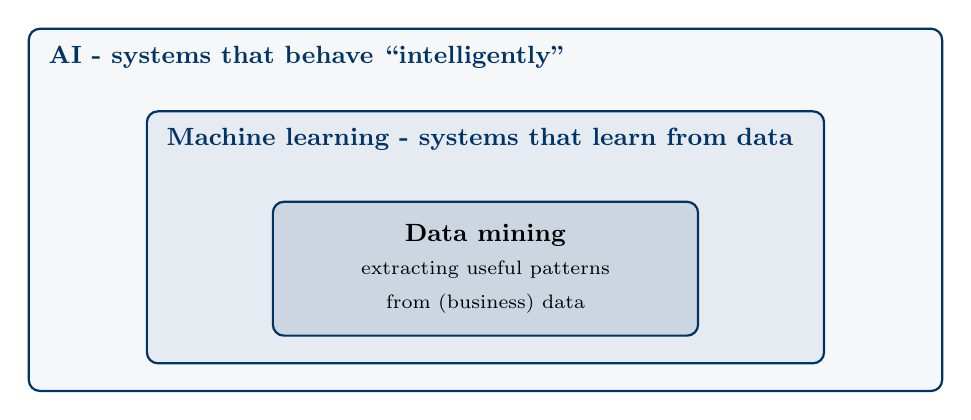
\begin{tikzpicture}[
      lab/.style={font=\small\bfseries, text=sghblue},
      box/.style={draw=sghblue, thick, rounded corners, align=center}]
    \node[box, minimum width=11.6cm, minimum height=4.6cm, fill=sghblue!4] (ai) {};
    \node[lab, anchor=north west] at ([xshift=4pt,yshift=-3pt]ai.north west) {AI - systems that behave ``intelligently''};
    \node[box, minimum width=8.6cm, minimum height=3.2cm, fill=sghblue!10, anchor=south] at ([yshift=10pt]ai.south) (ml) {};
    \node[lab, anchor=north west] at ([xshift=4pt,yshift=-3pt]ml.north west) {Machine learning - systems that learn from data};
    \node[box, minimum width=5.4cm, minimum height=1.7cm, fill=sghblue!20, anchor=south] at ([yshift=10pt]ml.south) (dm) {\small\textbf{Data mining}\\\scriptsize extracting useful patterns\\\scriptsize from (business) data};
  \end{tikzpicture}
  \end{center}
  \vspace{0.2em}
  \begin{itemize}\small
    \item \textbf{Statistics} underpins all three rings: inference, uncertainty, experimental design.
    \item In practice the borders are soft - employers say ``data science'' and mean the union.
  \end{itemize}
\end{frame}

% ---------------------------------------------------------------
\begin{frame}{Three ways a machine can learn}
  \begin{columns}[T]
    \begin{column}{0.32\textwidth}
      \textbf{Supervised}
      \begin{itemize}\small
        \item data comes with \alert{labels}
        \item learn to predict the label for new cases
        \item \emph{will this customer default?}
      \end{itemize}
    \end{column}
    \begin{column}{0.32\textwidth}
      \textbf{Unsupervised}
      \begin{itemize}\small
        \item no labels - find \alert{structure}
        \item clusters, patterns, compressed representations
        \item \emph{which customers are similar?}
      \end{itemize}
    \end{column}
    \begin{column}{0.32\textwidth}
      \textbf{Reinforcement}
      \begin{itemize}\small
        \item an agent acts, gets \alert{rewards}, adapts
        \item \emph{which collections action to try next?}
      \end{itemize}
    \end{column}
  \end{columns}
  \vspace{0.8em}
  \begin{center}\small
    This course: \textbf{supervised} (Blocks 2--3, 6) and \textbf{unsupervised}
    (Blocks 4--5). Reinforcement learning we only mention - so you know
    where it sits on the map.
  \end{center}
\end{frame}

% ---------------------------------------------------------------
\begin{frame}{Supervised learning comes in flavours}
  \small
  \begin{center}
  \begin{tabular}{@{}lp{4.2cm}p{4.6cm}@{}}
    \toprule
    Task & Target & Credit example \\
    \midrule
    \textbf{Binary classification} & two classes & \texttt{default} $\in \{0,1\}$ \\
    \textbf{Multiclass classification} & several classes & complaint category; rating grade \\
    \textbf{Regression} & a number & loss amount; recovery rate \\
    \emph{\ldots and more} & ordinal, ranking, survival time & months until default \\
    \bottomrule
  \end{tabular}
  \end{center}
  \vspace{0.7em}
  \begin{center}
    Our focus: \alert{binary classification} and \alert{regression}.\\
    The rest we will meet in passing - enough to recognise them in the wild.
  \end{center}
\end{frame}

% ---------------------------------------------------------------
\begin{frame}{From business question to learning task}
  \small
  \begin{center}
  \begin{tabular}{@{}p{5.6cm}p{3.4cm}p{3.4cm}@{}}
    \toprule
    Business question & Learning task & Covered in \\
    \midrule
    Will this applicant default? & binary classification & Blocks 2--3, 6 \\
    How large will the loss be if they do? & regression & Blocks 2--3 \\
    Which complaint team should read this email? & multiclass classification & Block 5 (mention) \\
    Do our customers form natural segments? & clustering & Block 4 \\
    Which products are bought together? & association rules & Block 5 \\
    \bottomrule
  \end{tabular}
  \end{center}
  \vspace{0.6em}
  \begin{center}
    The translation step is \alert{your} job - no algorithm does it for you.\\
    \small Getting it wrong here invalidates everything downstream.
  \end{center}
\end{frame}

% ---------------------------------------------------------------
\begin{frame}{The spine of the course: CRISP-DM}
  \centering
  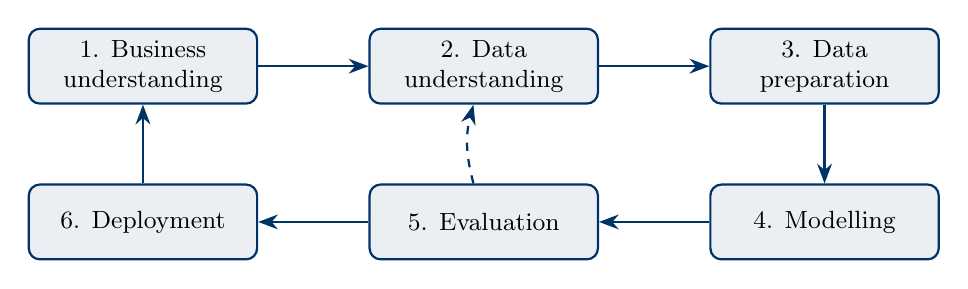
\begin{tikzpicture}[
      node distance=1.0cm and 1.4cm,
      box/.style={draw=sghblue,thick,rounded corners,fill=sghblue!8,
                  minimum width=2.9cm,minimum height=0.95cm,align=center,font=\small},
      ar/.style={-{Stealth[length=2.5mm]},sghblue,thick}]
    \node[box] (biz) {1. Business\\understanding};
    \node[box,right=of biz] (data) {2. Data\\understanding};
    \node[box,right=of data] (prep) {3. Data\\preparation};
    \node[box,below=of prep] (model) {4. Modelling};
    \node[box,left=of model] (eval) {5. Evaluation};
    \node[box,left=of eval] (deploy) {6. Deployment};
    \draw[ar] (biz) -- (data);
    \draw[ar] (data) -- (prep);
    \draw[ar] (prep) -- (model);
    \draw[ar] (model) -- (eval);
    \draw[ar] (eval) -- (deploy);
    \draw[ar] (deploy) -- (biz);
    \draw[ar,dashed] (eval) to[bend left=15] (data);
  \end{tikzpicture}
  \vspace{0.5em}
  \begin{center}\small Today lives in boxes \textbf{1 and 2}. The dashed arrow is the point:
  evaluation sends you back to understanding.\end{center}
\end{frame}

% ---------------------------------------------------------------
\begin{frame}{Where a project's time actually goes}
  \begin{center}
    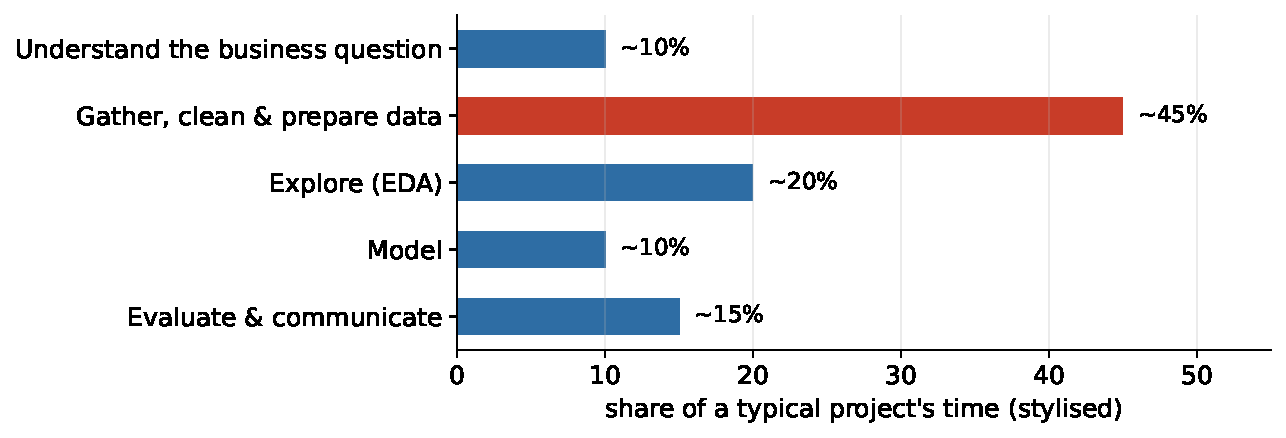
\includegraphics[width=0.8\textwidth]{figures/fig_time_split.pdf}
  \end{center}
  \begin{itemize}\small
    \item Modelling - the part courses spend most time on - is a
          \alert{small slice} of real work.
    \item That is why this course starts with data understanding, not with
          algorithms.
  \end{itemize}
\end{frame}

% ---------------------------------------------------------------
\begin{frame}{Our business problem for the whole term}
  \begin{block}{The lender's question}
    Given what we know about a customer at application time, how likely are they
    to \alert{default}? And what should we \emph{do} about it?
  \end{block}
  \begin{itemize}\small
    \item Each row = one credit customer; target \texttt{default} $\in \{0,1\}$.
    \item Realistic ingredients: income, debt-to-income, utilisation, prior
          delinquency, existing loans, savings, purpose\ldots
    \item Realistic problems: \alert{class imbalance}, \alert{missing data},
          and \alert{leakage} - all of which we meet today or next week.
  \end{itemize}
  \vspace{0.4em}
  \begin{center}\small Today: the synthetic portfolio via \texttt{finance\_data.load\_credit()};
  from Block~2, the real Taiwan portfolio via \texttt{load\_taiwan()} - same lender's question.\end{center}
\end{frame}

% ---------------------------------------------------------------
\begin{frame}{First decision nobody teaches: what is a \emph{row}?}
  \textbf{The unit of analysis} - what one row of your table represents:
  \begin{itemize}\small
    \item one \textbf{application}? \quad one \textbf{customer}? \quad one
          \textbf{customer-month}? \quad one \textbf{transaction}?
  \end{itemize}
  \vspace{0.5em}
  \textbf{Why it matters}
  \begin{itemize}\small
    \item The unit fixes what the prediction \emph{means} - and when it can be used.
    \item A customer with 3 loans: three rows or one? Your metrics change either way.
    \item Mixing units (some rows customers, some applications) silently
          \alert{double-counts} people.
  \end{itemize}
  \vspace{0.5em}
  \begin{center}
    In our portfolio: one row = one \alert{customer with one loan application}.
  \end{center}
\end{frame}

% ---------------------------------------------------------------
\begin{frame}{Meet the dataset}
  \footnotesize
  \begin{center}
  \begin{tabular}{@{}lll@{}}
    \toprule
    Column (sample) & Type & Notes \\
    \midrule
    \texttt{customer\_id} & identifier & never a feature! \\
    \texttt{age}, \texttt{monthly\_income\_pln} & numeric & income has missing values \\
    \texttt{housing}, \texttt{purpose}, \texttt{region} & categorical & no natural order \\
    \texttt{checking\_status} & categorical (ordinal) & none $<$ low $<$ medium $<$ high \\
    \texttt{credit\_utilization}, \texttt{debt\_to\_income} & numeric ratios & key risk drivers \\
    \texttt{months\_since\_last\_delinquency} & numeric & \alert{structurally missing} \\
    \texttt{collections\_contact} & 0/1 & \alert{a trap} - more in Block 3 \\
    \texttt{default} & 0/1 & the target \\
    \bottomrule
  \end{tabular}
  \end{center}
  \vspace{0.4em}
  \begin{center}\small 4{,}000 customers, 18 columns; German Credit (OpenML) or a
  synthetic Polish portfolio - same interface.\end{center}
\end{frame}

% ---------------------------------------------------------------
\begin{frame}{The data you will never see: selection bias}
  \begin{block}{Ask of every dataset: how did rows get \emph{into} this table?}
    A lender's portfolio contains only \alert{approved} loans. Rejected
    applicants have no \texttt{default} outcome - they are simply absent.
  \end{block}
  \vspace{0.4em}
  \begin{itemize}\small
    \item Our model learns on the \emph{survivors of yesterday's policy} -
          a form of survivorship bias.
    \item For applicants unlike anyone previously approved, the model
          \alert{extrapolates} - its confidence there is borrowed, not earned.
    \item Credit scoring has a name and a toolbox for this
          (\emph{reject inference}); most other domains quietly ignore it.
    \item Same pattern everywhere: churn models see only acquired customers,
          hiring models see only past hires.
  \end{itemize}
  \vspace{0.4em}
  \begin{center}
    Selection bias cannot be fixed by more data \alert{from the same source}.
  \end{center}
\end{frame}

% ============================================================
% SECTION: EDA
% ============================================================
\section{EDA}

% ---------------------------------------------------------------
\begin{frame}{Before any model: look at the data}
  \textbf{Data understanding checklist}
  \begin{enumerate}\small
    \item Shape, columns, data types.
    \item Target balance - how (im)balanced is \texttt{default}?
    \item Univariate: distributions, implausible values, units.
    \item Bivariate: which features move with the target?
    \item \alert{Data quality}: duplicates, outliers, and \emph{missingness}.
  \end{enumerate}
  \vspace{0.5em}
  \begin{center}
    Skipping this step is the most common way a data-mining project quietly fails.
  \end{center}
\end{frame}

% ---------------------------------------------------------------
\begin{frame}[fragile]{First contact with a DataFrame}
\small Four commands before anything else:
{\footnotesize
\begin{semiverbatim}
df.shape                  \textit{\# how much data do I have?}
df.dtypes                 \textit{\# what does pandas think each column is?}
df.head(10)               \textit{\# do the values look like the docs promised?}
df.describe(include="all")  \textit{\# ranges, counts, uniques, NaNs}
\end{semiverbatim}}
  \vspace{0.4em}
  \textbf{What you are looking for}
  \begin{itemize}\small
    \item numbers stored as strings (\texttt{"12 000"}, \texttt{"N/A"}, \texttt{"-"})
    \item categorical levels that differ only by case or spelling
    \item minima / maxima that make no physical sense
    \item a \texttt{describe()} count smaller than \texttt{len(df)} - that is missingness
  \end{itemize}
\end{frame}

% ---------------------------------------------------------------
\begin{frame}[fragile]{Duplicates and keys}
  \textbf{Two questions for every table}
  \begin{itemize}\small
    \item What \emph{should} uniquely identify a row? (the key - here:
          \texttt{customer\_id})
    \item Does it? \quad
          {\footnotesize\texttt{df["customer\_id"].is\_unique}}
  \end{itemize}
  \vspace{0.4em}
  \textbf{Where duplicates come from}
  \begin{itemize}\small
    \item repeated exports glued together; joins that multiplied rows;
          customers applying twice
  \end{itemize}
  \vspace{0.4em}
  \textbf{Why it is dangerous}
  \begin{itemize}\small
    \item duplicated rows are double-counted evidence - metrics look
          better/worse than reality
    \item a duplicate that lands in both train and test set \alert{inflates
          every score} (a leakage cousin - Block 3)
  \end{itemize}
\end{frame}

% ---------------------------------------------------------------
\begin{frame}{Know your variable types}
  \small
  \begin{center}
  \begin{tabular}{@{}llp{4.8cm}@{}}
    \toprule
    Type & Example & Watch out for \\
    \midrule
    Numeric, continuous & income, DTI & skew, outliers, units \\
    Numeric, discrete & \# existing loans & often better treated as categories \\
    Categorical, nominal & purpose, region & rare levels, typos, encodings \\
    Categorical, ordinal & checking status & order matters - keep it \\
    Dates \& times & application date & time zones; enables leakage \\
    Text & complaint narrative & needs its own pipeline (Block 5) \\
    Identifiers & \texttt{customer\_id} & \alert{never} a feature \\
    \bottomrule
  \end{tabular}
  \end{center}
  \vspace{0.5em}
  \begin{center}
    The type decides the plot, the summary statistic, \emph{and} the encoding.
  \end{center}
\end{frame}

% ---------------------------------------------------------------
\begin{frame}{Scales of measurement (Stevens)}
  \small
  \begin{center}
  \begin{tabular}{@{}llll@{}}
    \toprule
    Scale & Defining property & Meaningful ops & Example \\
    \midrule
    \textbf{Nominal} & categories, no order & $=$, $\neq$ & purpose, region \\
    \textbf{Ordinal} & ordered, gaps unknown & $<$, $>$ & checking status \\
    \textbf{Interval} & equal gaps, no true zero & $+$, $-$ & temperature in °C; dates \\
    \textbf{Ratio} & true zero exists & $\times$, $\div$ & income, loan amount, age \\
    \bottomrule
  \end{tabular}
  \end{center}
  \vspace{0.6em}
  \textbf{Why it matters}
  \begin{itemize}\small
    \item The scale limits the statistics: a \alert{mean of nominal codes is
          nonsense}; medians need at least ordinal.
    \item ``Twice as much'' needs a ratio scale: 40°C is not twice as warm as
          20°C, but a 40k loan \emph{is} twice a 20k loan.
    \item Encoding an ordinal variable as one-hot throws its order away;
          encoding a nominal one as integers invents an order that isn't there.
  \end{itemize}
\end{frame}

% ---------------------------------------------------------------
\begin{frame}{The target comes first: class balance}
  \begin{center}
    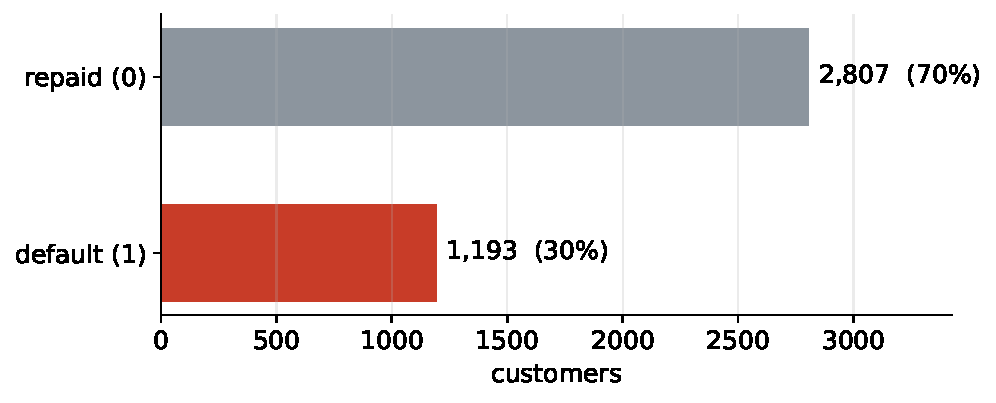
\includegraphics[width=0.8\textwidth]{figures/fig_target_balance.pdf}
  \end{center}
  \vspace{0.2em}
  \begin{itemize}\small
    \item A model that always says ``repaid'' is right 7 times out of 10 -
          and completely \alert{useless}.
    \item Accuracy is therefore \emph{not} the metric for imbalanced problems
          (proper treatment in Block 3).
    \item Real PD portfolios are far more extreme: 1--5\% default rates.
  \end{itemize}
\end{frame}

% ---------------------------------------------------------------
\begin{frame}{Univariate EDA: the shape of a distribution}
  \begin{center}
    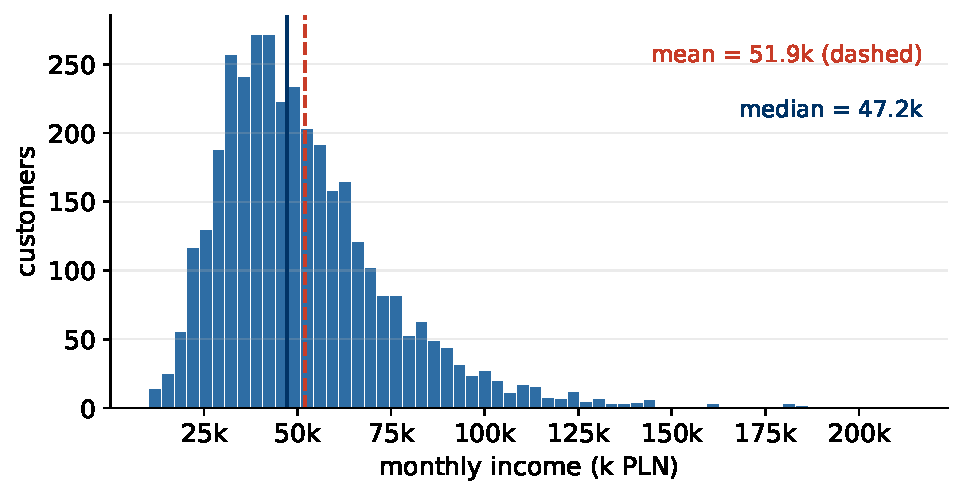
\includegraphics[width=0.74\textwidth]{figures/fig_income_hist.pdf}
  \end{center}
  \begin{itemize}\small
    \item Income is \alert{right-skewed}: mean $>$ median - a few high earners
          pull the mean up.
    \item Skew is information: it tells you which summary to report and
          whether a transform will help.
  \end{itemize}
\end{frame}

% ---------------------------------------------------------------
\begin{frame}{Heavy tails? Change the lens}
  \begin{center}
    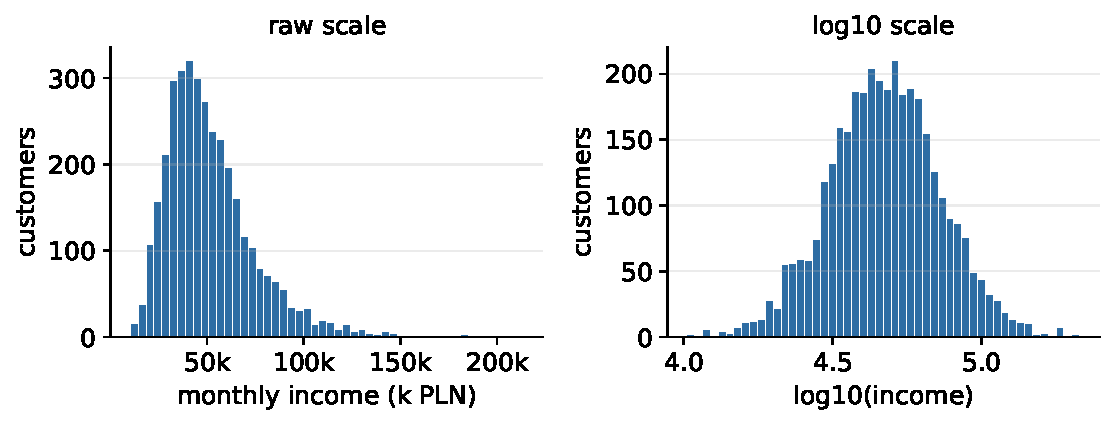
\includegraphics[width=0.9\textwidth]{figures/fig_income_log.pdf}
  \end{center}
  \begin{itemize}\small
    \item On a log scale the same variable becomes nearly symmetric.
    \item Monetary amounts (income, savings, loss) almost always deserve a
          log look - \alert{multiplicative} thinking fits money.
  \end{itemize}
\end{frame}

% ---------------------------------------------------------------
\begin{frame}{Sanity checks: implausible values}
  \small
  \begin{center}
  \begin{tabular}{@{}lp{4.6cm}p{4.2cm}@{}}
    \toprule
    Red flag & Example & Likely cause \\
    \midrule
    Impossible values & age $= 150$; income $< 0$ & entry error, sentinel codes \\
    Sentinel numbers & income $= 999999$ & ``missing'' coded as a number \\
    Unit mixes & salary 3{,}000 vs 36{,}000 & monthly vs annual, PLN vs EUR \\
    Too-round values & everyone earns exactly 5{,}000 & defaults filled by a form \\
    Frozen columns & one value everywhere & broken export, dead field \\
    \bottomrule
  \end{tabular}
  \end{center}
  \vspace{0.5em}
  \begin{center}
    Every red flag is a \alert{question for the data owner}, not a value to
    silently ``fix''.
  \end{center}
\end{frame}

% ---------------------------------------------------------------
\begin{frame}{Categoricals: levels and rare categories}
  \begin{center}
    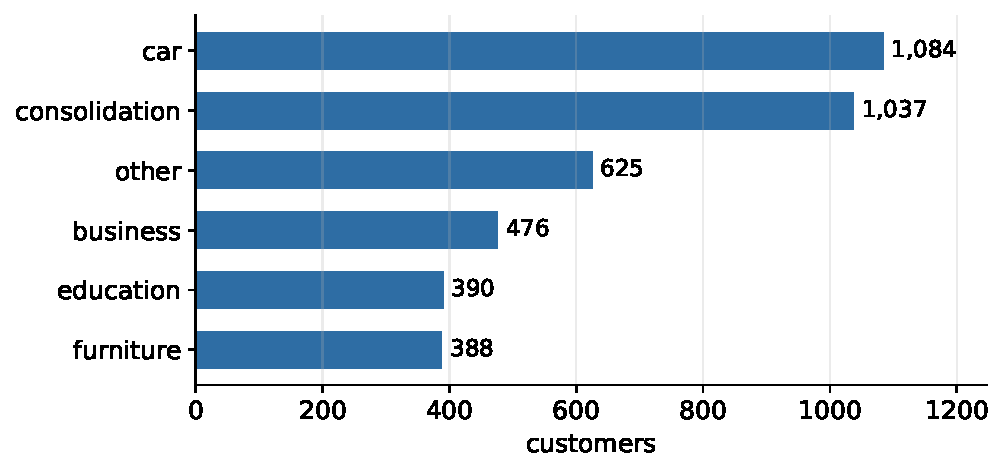
\includegraphics[width=0.72\textwidth]{figures/fig_purpose_counts.pdf}
  \end{center}
  \begin{itemize}\small
    \item Check levels: typos and case variants create phantom categories.
    \item Rare levels ($<$1--2\% of rows) often get grouped into
          \texttt{other} - but only \emph{after} checking they are not
          special (e.g.\ a tiny, very risky segment).
  \end{itemize}
\end{frame}

% ---------------------------------------------------------------
\begin{frame}{Bivariate EDA: numeric feature vs target}
  \begin{center}
    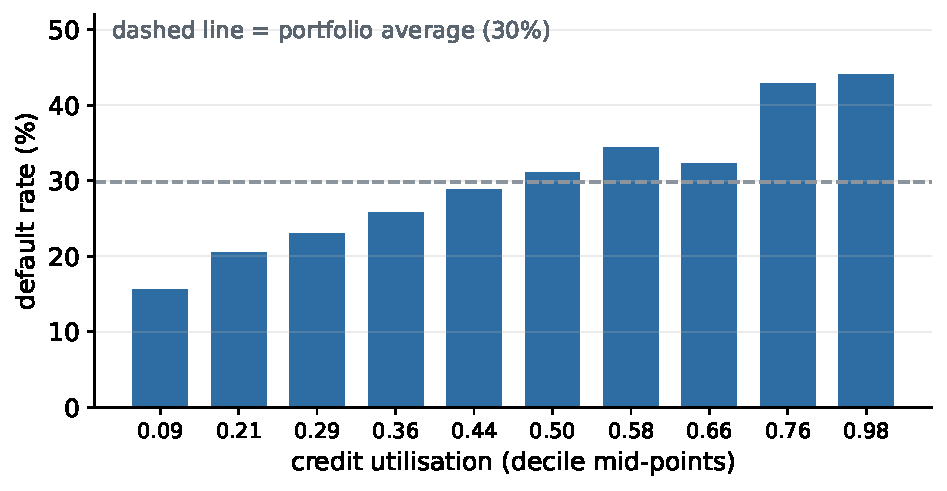
\includegraphics[width=0.74\textwidth]{figures/fig_default_by_utilization.pdf}
  \end{center}
  \begin{itemize}\small
    \item Bin the feature, plot the default rate per bin - the
          \alert{shape} of the risk relationship appears.
    \item Monotone and steep $\Rightarrow$ a strong candidate feature
          (utilisation is a classic credit driver).
  \end{itemize}
\end{frame}

% ---------------------------------------------------------------
\begin{frame}{Bivariate EDA: categorical feature vs target}
  \begin{center}
    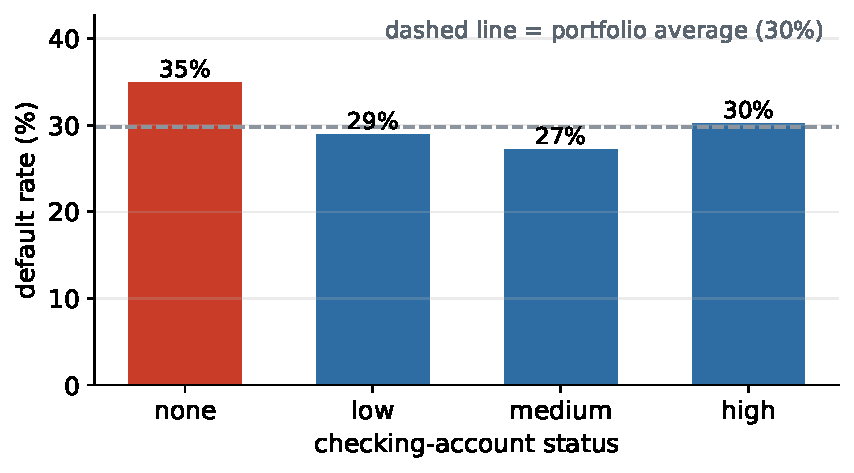
\includegraphics[width=0.64\textwidth]{figures/fig_default_by_checking.pdf}
  \end{center}
  \begin{itemize}\small
    \item ``No checking account'' is the riskiest group - the bank cannot
          see those customers' cash flows.
    \item Compare each level to the \emph{portfolio average}, and mind small
          groups: a rate computed on 30 customers is noise.
  \end{itemize}
\end{frame}

% ---------------------------------------------------------------
\begin{frame}{A first map: the correlation matrix}
  \begin{columns}[T]
    \begin{column}{0.58\textwidth}
      \begin{center}
        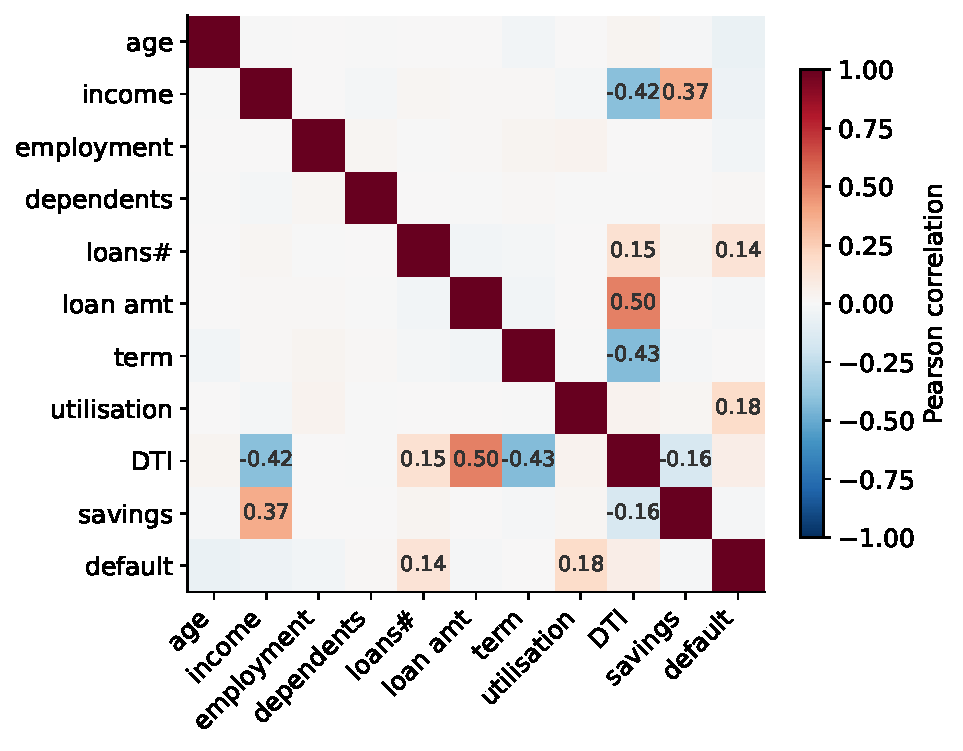
\includegraphics[height=0.78\textheight]{figures/fig_corr_heatmap.pdf}
      \end{center}
    \end{column}
    \begin{column}{0.4\textwidth}
      \vspace{1.2em}
      \begin{itemize}\small
        \item One picture: which features move together, and which move
              with the target.
        \item Utilisation and the number of existing loans stand out for
              \texttt{default} - current debt load beats income here.
        \item Strongly correlated feature pairs ($|r| > 0.8$) are candidates
              for dropping one.
      \end{itemize}
    \end{column}
  \end{columns}
\end{frame}

% ---------------------------------------------------------------
\begin{frame}{Correlation: handle with care}
  \begin{itemize}
    \item \textbf{Correlation is not causation.} Ice cream sales correlate
          with drownings; summer causes both.
    \item \textbf{Pearson sees only straight lines.} A perfect U-shaped
          relationship can have $r \approx 0$.
    \item \textbf{Outliers can manufacture correlation.} One extreme point can
          turn $r = 0.1$ into $r = 0.7$.
    \item \textbf{Rank alternatives exist.} Spearman correlation asks only
          ``do they move in the same direction?'' - more robust for skewed data.
  \end{itemize}
  \vspace{0.6em}
  \begin{center}
    A correlation matrix generates \alert{hypotheses}, not conclusions.
  \end{center}
\end{frame}

% ---------------------------------------------------------------
\begin{frame}{Simpson's paradox: the aggregate can lie}
  \begin{center}
    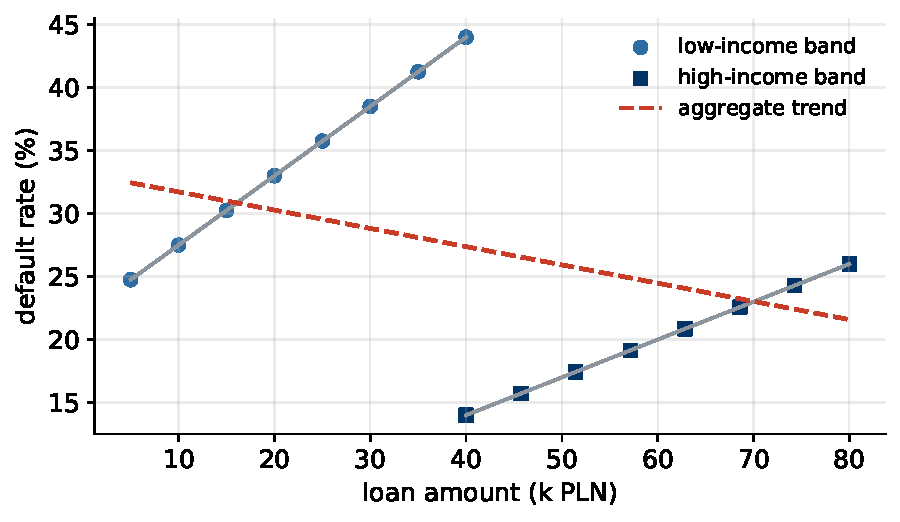
\includegraphics[width=0.62\textwidth]{figures/fig_simpson.pdf}
  \end{center}
  \begin{itemize}\small
    \item In aggregate, bigger loans look \emph{safer} - because high-income
          customers take the big loans.
    \item Within \emph{every} income band, bigger loans are riskier.
          Both statements are true; only one is useful.
    \item Before concluding from any bivariate plot, ask:
          \alert{compared within what?} (Illustrative data.)
  \end{itemize}
\end{frame}

% ---------------------------------------------------------------
\begin{frame}{Why you must plot: Anscombe's quartet}
  \begin{center}
    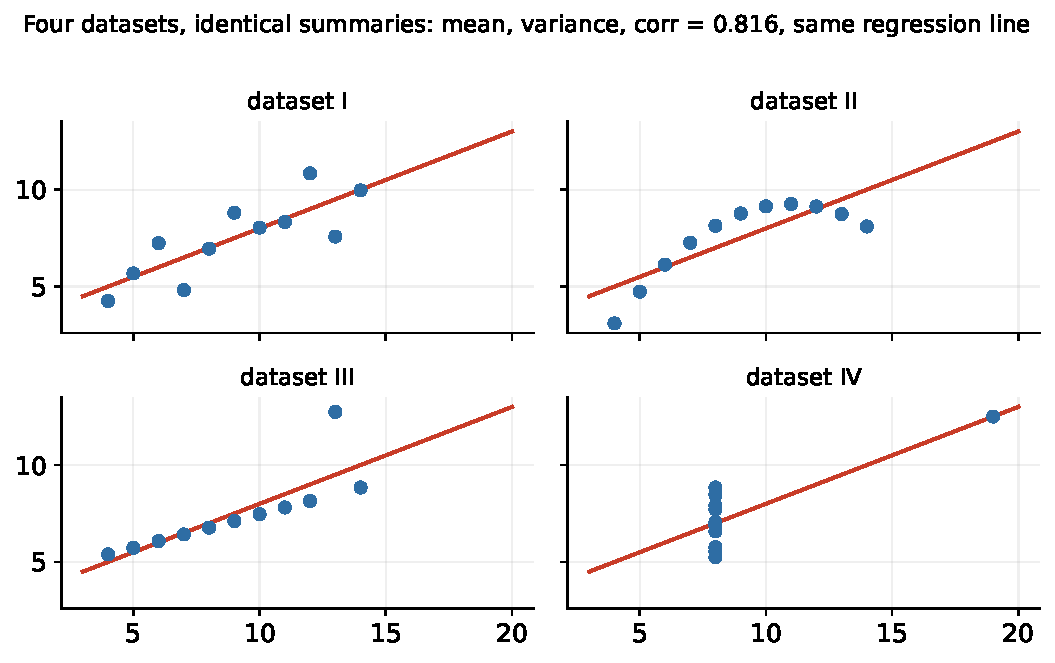
\includegraphics[width=0.6\textwidth]{figures/fig_anscombe.pdf}
  \end{center}
  \begin{center}\small
    Same mean, same variance, same correlation, same regression line -
    four completely different stories. \alert{Summary statistics hide; plots reveal.}
  \end{center}
\end{frame}

% ---------------------------------------------------------------
\begin{frame}{Outliers: how to spot them}
  \begin{center}
    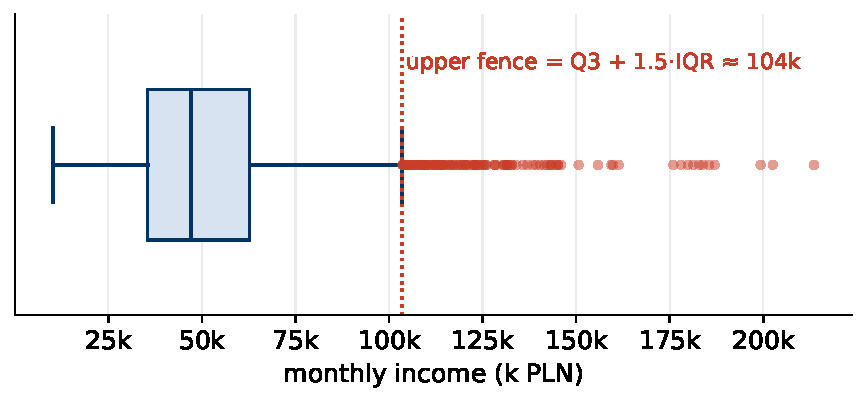
\includegraphics[width=0.76\textwidth]{figures/fig_outliers_box.pdf}
  \end{center}
  \begin{itemize}\small
    \item The boxplot's \textbf{IQR rule}: flag points beyond
          $Q3 + 1.5\cdot\text{IQR}$ (or below $Q1 - 1.5\cdot\text{IQR}$).
    \item A convention, not a law - for skewed variables it flags many
          perfectly genuine values (log first, then look again).
  \end{itemize}
\end{frame}

% ---------------------------------------------------------------
\begin{frame}{Outliers: what to actually do}
  \begin{enumerate}
    \item \textbf{Investigate first.} Error or real? A 2 mln PLN income might
          be a typo - or a real customer who matters.
    \item \textbf{If it is an error}: fix from source, or set to missing
          (do not invent a value).
    \item \textbf{If it is genuine}: keep it; consider capping / winsorising
          or a log transform so it stops dominating.
    \item \textbf{Document the rule} - ``we capped income at the 99th
          percentile'' must be written down and applied identically to new data.
  \end{enumerate}
  \vspace{0.5em}
  \begin{alertblock}{Fraud-detection perspective}
    In fraud, outliers are not noise - they are often \emph{the signal}.
    Whether an outlier is a problem depends on the business question.
  \end{alertblock}
\end{frame}

% ---------------------------------------------------------------
\begin{frame}{EDA is a loop, not a phase}
  \begin{columns}[T]
    \begin{column}{0.5\textwidth}
      \textbf{The rhythm}
      \begin{enumerate}\small
        \item ask a question
        \item make the one plot that answers it
        \item the answer raises two new questions
        \item repeat until surprises stop
      \end{enumerate}
    \end{column}
    \begin{column}{0.5\textwidth}
      \textbf{Keep an evidence log}
      \begin{itemize}\small
        \item every finding: one sentence + the plot
        \item ``income is MNAR-missing for high earners'' beats
              40 unlabelled histograms
        \item your future self (and your team) will re-read it
      \end{itemize}
    \end{column}
  \end{columns}
  \vspace{0.7em}
  \begin{center}
    EDA never really ends - evaluation (CRISP-DM's dashed arrow) sends you
    back here.
  \end{center}
\end{frame}

% ============================================================
% SECTION: DATA QUALITY & MISSINGNESS
% ============================================================
\section{Missingness}

% ---------------------------------------------------------------
\begin{frame}{Missing data is not one thing}
  \small
  \begin{center}
  \begin{tabular}{@{}lp{5.0cm}p{4.2cm}@{}}
    \toprule
    Type & Meaning & Credit example \\
    \midrule
    \textbf{MCAR} & missing completely at random & a system glitch drops a field \\
    \textbf{MAR}  & depends on \emph{observed} data & renters skip employment length \\
    \textbf{MNAR} & depends on the \emph{unobserved} value & high earners hide income \\
    \textbf{Structural} & the value cannot exist & ``months since last delinquency'' when there was none \\
    \bottomrule
  \end{tabular}
  \end{center}
  \vspace{0.7em}
  \begin{center}
    The \alert{mechanism} decides whether it is safe to drop, impute, or \emph{model}.
  \end{center}
\end{frame}

% ---------------------------------------------------------------
\begin{frame}{Our portfolio: how much is missing, and why}
  \begin{center}
    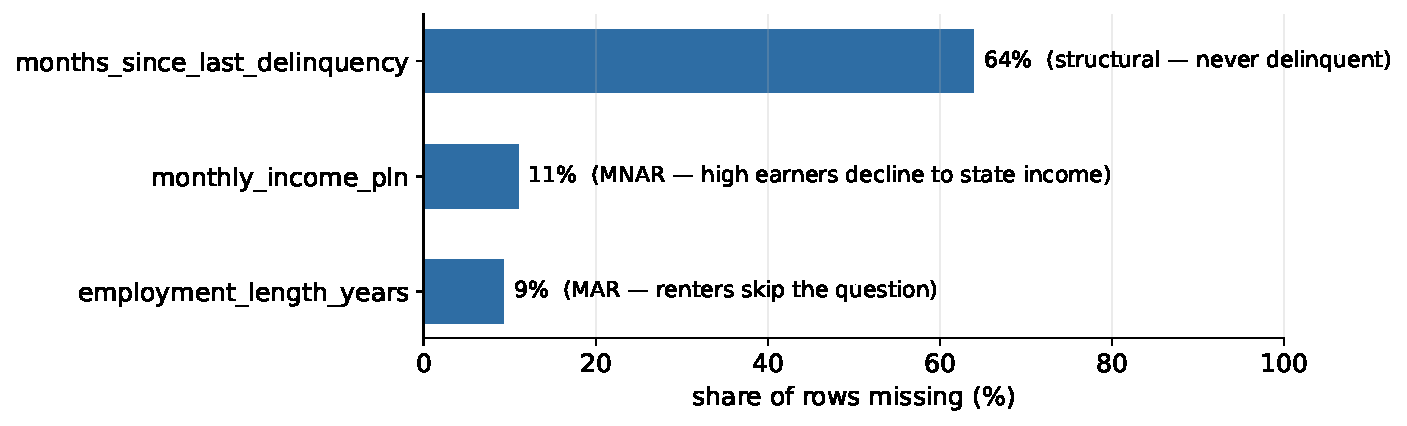
\includegraphics[width=0.95\textwidth]{figures/fig_missingness.pdf}
  \end{center}
  \begin{itemize}\small
    \item Three columns, three different mechanisms - and three different
          correct treatments.
    \item First step is always the same: \alert{count and name} the
          missingness before touching it.
  \end{itemize}
\end{frame}

% ---------------------------------------------------------------
\begin{frame}{Seeing the pattern of missingness}
  \begin{center}
    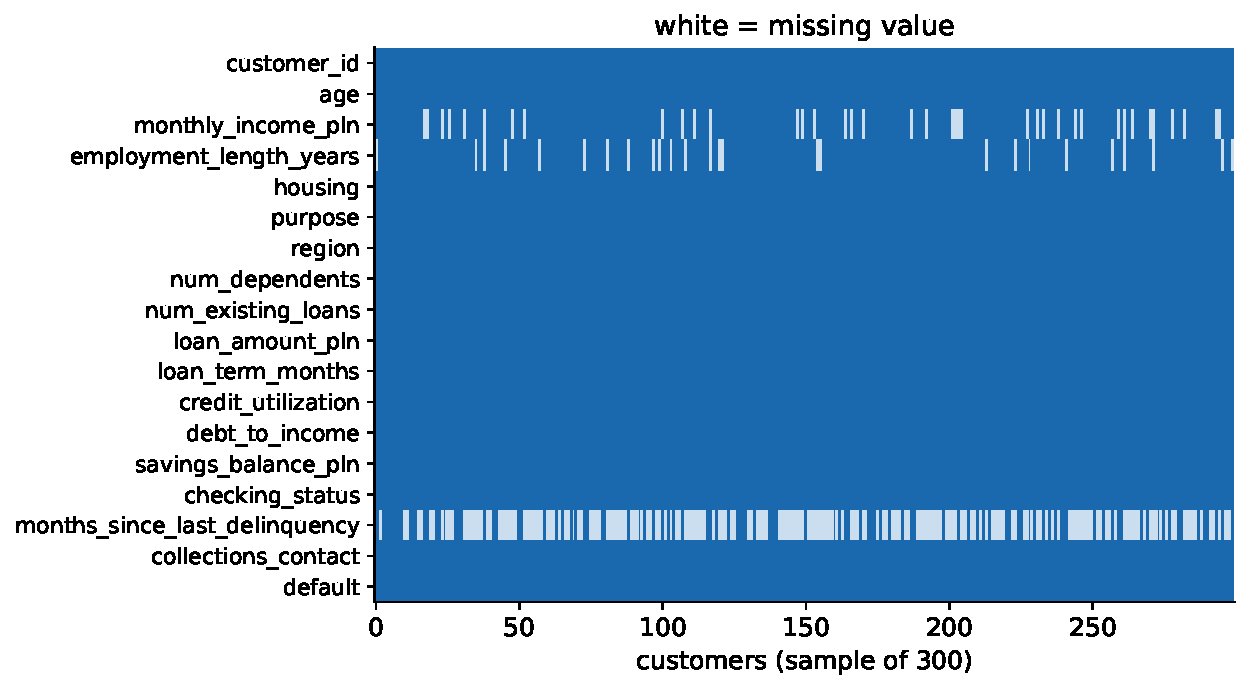
\includegraphics[width=0.66\textwidth]{figures/fig_missing_matrix.pdf}
  \end{center}
  \begin{itemize}\small
    \item A missingness matrix shows \emph{structure}: which columns, how
          often, and whether gaps co-occur in the same rows.
    \item In the lab: the same view via \texttt{df.isna()} - no extra
          library needed.
  \end{itemize}
\end{frame}

% ---------------------------------------------------------------
\begin{frame}{Option 1: deletion - when dropping is (not) safe}
  \textbf{Dropping rows (listwise deletion)}
  \begin{itemize}\small
    \item Safe-ish only under \textbf{MCAR} - you lose power, but no bias.
    \item Under MAR/MNAR it \alert{biases the sample}: dropping
          income-missing rows here removes high earners.
  \end{itemize}
  \vspace{0.4em}
  \textbf{Dropping columns}
  \begin{itemize}\small
    \item Defensible when a column is mostly empty \emph{and} carries no
          signal - check both.
    \item Here, \texttt{months\_since\_last\_delinquency} is $\sim$64\% missing and
          still one of the \alert{most informative} columns in the data.
  \end{itemize}
  \vspace{0.5em}
  \begin{center}
    Deletion is a modelling decision, not housekeeping - justify it like one.
  \end{center}
\end{frame}

% ---------------------------------------------------------------
\begin{frame}{Option 2: the imputation menu}
  \small
  \begin{center}
  \begin{tabular}{@{}lp{4.4cm}p{4.4cm}@{}}
    \toprule
    Method & Good & Risky \\
    \midrule
    Mean / median & simple, fast; median survives skew & shrinks variance; distorts under MAR/MNAR \\
    Mode (categorical) & simple & inflates the majority level \\
    Group-wise median & respects segments (e.g.\ per region) & groups must be big enough \\
    Model-based / KNN & uses relationships between features & complexity, leakage risk if fit on all data \\
    Constant + \textbf{indicator} & keeps ``was missing'' as signal & adds columns \\
    \bottomrule
  \end{tabular}
  \end{center}
  \vspace{0.4em}
  \begin{center}
    Golden rule: fit any imputation on the \alert{training data only} -
    a preview of Block 3's leakage discussion.
  \end{center}
\end{frame}

% ---------------------------------------------------------------
\begin{frame}{A missing value can be a signal}
  \begin{center}
    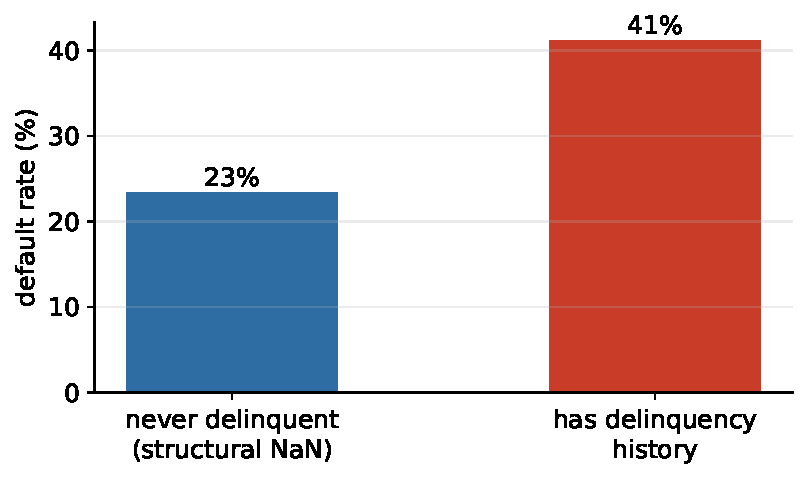
\includegraphics[width=0.62\textwidth]{figures/fig_structural_signal.pdf}
  \end{center}
  \begin{itemize}\small
    \item Customers with the structural NaN (never delinquent) default far
          less often - the \alert{gap itself predicts}.
    \item Any treatment that erases the gap erases the signal.
  \end{itemize}
\end{frame}

% ---------------------------------------------------------------
\begin{frame}{The punchline of Block 1}
  \begin{block}{A missing value can be the strongest signal you have}
    Customers with \emph{no prior delinquency} carry a structural NaN in
    ``months since last delinquency''. Mean-imputing it would \alert{invent a
    delinquency history that never happened} - and erase a real signal.
  \end{block}
  \begin{itemize}\small
    \item Honest first move: add a \textbf{missing-indicator}, \emph{then} impute the number.
    \item In regulated lending, the reason you give a customer must be truthful.
          Imputation choices are not cosmetic - they change the story.
  \end{itemize}
\end{frame}

% ---------------------------------------------------------------
\begin{frame}{A first warning about leakage}
  \begin{block}{Leakage = using information that will not exist at prediction time}
    Our dataset contains \texttt{collections\_contact} - whether collections
    called the customer. It is \alert{recorded after default happens}. A model
    using it looks brilliant in the notebook and is worthless in production.
  \end{block}
  \vspace{0.4em}
  \textbf{The time-travel test (ask for every feature):}
  \begin{center}
    \emph{``Would I have known this value at the moment of the decision?''}
  \end{center}
  \vspace{0.4em}
  \begin{itemize}\small
    \item If the answer is no - the feature is a time traveller. Drop it.
    \item Full treatment (and a live demonstration) in Block 3.
  \end{itemize}
\end{frame}

% ============================================================
% SECTION: FEATURE ENGINEERING
% ============================================================
\section{Features}

% ---------------------------------------------------------------
\begin{frame}{Feature engineering: where domain knowledge becomes signal}
  New columns that expose structure the model would struggle to find alone.
  The missing-indicator you just built \emph{is} feature engineering -
  here is the wider toolbox:
  \vspace{0.3em}
  \small
  \begin{center}
  \begin{tabular}{@{}llp{4.6cm}@{}}
    \toprule
    Move & Recipe & Portfolio example \\
    \midrule
    \textbf{Ratio} & divide two raw columns & instalment / income \\
    \textbf{Flag} & boolean condition & \texttt{has\_delinquency\_history} \\
    \textbf{Binning} & continuous $\to$ bands & utilisation: low / mid / maxed-out \\
    \textbf{Interaction} & combine two features & renter \emph{and} no checking account \\
    \textbf{Date arithmetic} & differences, tenures & months since last delinquency \\
    \bottomrule
  \end{tabular}
  \end{center}
  \vspace{0.4em}
  \begin{center}\small
    Look at the data dictionary again: \texttt{debt\_to\_income} is a ratio -
    \alert{someone engineered it before us}.
  \end{center}
\end{frame}

% ---------------------------------------------------------------
\begin{frame}{Worked example: combining two weak flags}
  \begin{center}
    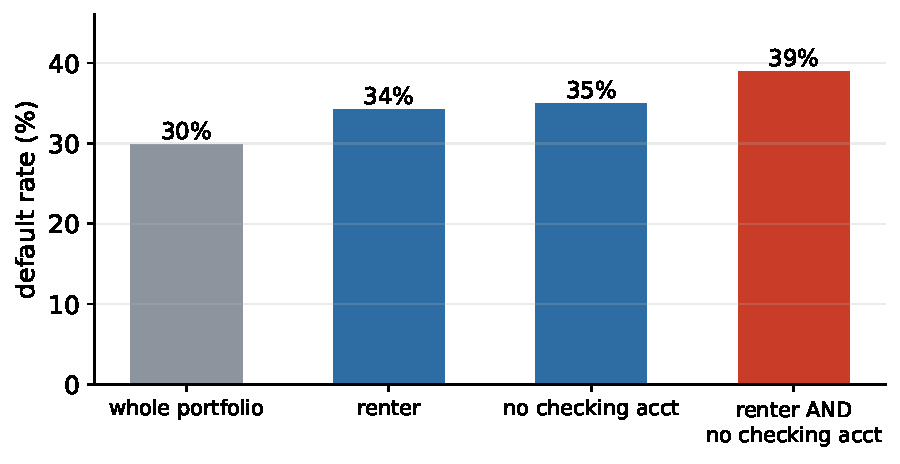
\includegraphics[width=0.66\textwidth]{figures/fig_interaction.pdf}
  \end{center}
  \begin{itemize}\small
    \item Renting alone and no-checking-account alone are each mildly risky;
          the \alert{interaction flag} isolates the riskiest segment (39\%,
          $n = 318$ - large enough to trust).
    \item And recall the strongest engineered feature so far: the
          \texttt{delinq\_missing} \alert{indicator} ($|r| \approx 0.19$ with
          default - more than any raw numeric column).
  \end{itemize}
\end{frame}

% ---------------------------------------------------------------
\begin{frame}{Feature engineering: rules of the game}
  \begin{enumerate}
    \item \textbf{Application-time information only} - every engineered
          feature must pass the \alert{time-travel test}, same as raw ones.
    \item \textbf{Fit transforms on training data only} - means for scaling,
          bin edges, encodings (the leakage-safe pipeline, Block 3).
    \item \textbf{Simple and explainable beats clever} - in regulated
          lending every feature may end up in an adverse-action reason.
    \item \textbf{Document the recipe} - production must compute the feature
          \emph{identically}, or the model silently degrades.
    \item \textbf{Expect diminishing returns} - five features built from
          domain sense beat five hundred generated blindly.
  \end{enumerate}
  \vspace{0.5em}
  \begin{center}\small
    Hands-on: exercise 5 in today's lab asks you to engineer one feature from
    loan amount, term, and income - and defend it.
  \end{center}
\end{frame}

% ---------------------------------------------------------------
\begin{frame}{Encodings: making categories digestible (preview)}
  Most models eat numbers, not labels. The scale of measurement picks the encoding:
  \vspace{0.3em}
  \footnotesize
  \begin{center}
  \begin{tabular}{@{}lll@{}}
    \toprule
    Encoding & Use for & Watch out for \\
    \midrule
    \textbf{One-hot} & nominal (purpose, region) & column explosion with many levels \\
    \textbf{Ordinal codes} & truly ordered (checking status) & only when the order is real \\
    \textbf{Target encoding} & high-cardinality nominal & \alert{leakage} - fit on train only \\
    \textbf{WoE} (credit tradition) & scorecard features & needs binning first; Block 2 \\
    \bottomrule
  \end{tabular}
  \end{center}
  \small
  \vspace{0.5em}
  \begin{itemize}\small
    \item Encoding nominal as integers invents an order; one-hot on ordinal
          discards one. \emph{Scale first, encoding second.}
    \item Full treatment next week, when regression needs numeric inputs.
  \end{itemize}
\end{frame}

% ============================================================
% SECTION: THE CRAFT
% ============================================================
\section{The craft}

% ---------------------------------------------------------------
\begin{frame}{Reproducibility from day one}
  \begin{itemize}
    \item \textbf{Fix your random seeds} - \texttt{random\_state=42}
          everywhere a coin is flipped (splits, models, samples).
    \item \textbf{Pin your environment} - \texttt{uv} lockfile; ``works on my
          machine'' is not a result.
    \item \textbf{One-command rule} - a colleague should reproduce your
          numbers by running one thing, top to bottom.
    \item \textbf{Data provenance} - record where the data came from and
          when; datasets change under your feet.
  \end{itemize}
  \vspace{0.6em}
  \begin{center}
    If it cannot be reproduced, it is an \alert{anecdote}, not an analysis -
    and the project rubric scores it.
  \end{center}
\end{frame}

% ---------------------------------------------------------------
\begin{frame}{Notebooks: superpower and trap}
  \begin{columns}[T]
    \begin{column}{0.5\textwidth}
      \textbf{Superpower}
      \begin{itemize}\small
        \item code + plots + narrative in one place
        \item perfect for EDA and for the project report
      \end{itemize}
    \end{column}
    \begin{column}{0.5\textwidth}
      \textbf{Trap: hidden state}
      \begin{itemize}\small
        \item cells run out of order $\Rightarrow$ results that cannot be
              recreated
        \item deleted cells leave live variables behind
      \end{itemize}
    \end{column}
  \end{columns}
  \vspace{0.7em}
  \begin{alertblock}{The habit that saves you}
    Before trusting any result: \textbf{Restart kernel \& run all}.
    If it breaks, it was already broken - you just didn't know.
  \end{alertblock}
\end{frame}

% ---------------------------------------------------------------
\begin{frame}{Version control - yes, for analysts too}
  \begin{itemize}
    \item \textbf{Commit small and often} - each commit one logical step;
          messages that say \emph{why}.
    \item \textbf{What goes in}: code, notebooks, configs, figure scripts.
    \item \textbf{What stays out}: raw data (use loaders), credentials,
          \texttt{.env} files, 100 MB artefacts.
    \item \textbf{Why bother in a student project?} You will want yesterday's
          working version at 23:50 before the deadline.
  \end{itemize}
  \vspace{0.6em}
  \begin{center}\small
    \texttt{git init} today costs 10 seconds. Reconstructing a deleted
    analysis costs a weekend.
  \end{center}
\end{frame}

% ---------------------------------------------------------------
\begin{frame}{Reading errors \& asking good questions}
  \textbf{When code explodes}
  \begin{itemize}\small
    \item Read the traceback \alert{bottom-up}: the last line is the error,
          the lines above are where it happened.
    \item Reproduce it in the smallest possible example - half the time the
          bug evaporates as you shrink it.
  \end{itemize}
  \vspace{0.5em}
  \textbf{When you ask for help} (colleague, forum, AI assistant)
  \begin{itemize}\small
    \item say what you expected, what happened instead, and what you tried
    \item include the minimal example - not a screenshot of 400 lines
    \item the discipline of writing the question well often \emph{answers} it
  \end{itemize}
\end{frame}

% ---------------------------------------------------------------
\begin{frame}{Communicating results to humans}
  \begin{itemize}
    \item \textbf{Lead with the decision}, not the method: ``we can cut losses
          12\% at the same approval rate'' beats ``our AUC is 0.79''.
    \item \textbf{State uncertainty honestly} - ranges and caveats build
          trust; false precision destroys it.
    \item \textbf{One chart, one message} - if a slide needs a paragraph of
          explanation, it is two slides.
    \item \textbf{Know your audience} - the risk committee, the regulator,
          and your fellow data scientist need three different stories.
  \end{itemize}
  \vspace{0.5em}
  \begin{center}
    Your model's impact is capped by your ability to \alert{explain} it.
  \end{center}
\end{frame}

% ---------------------------------------------------------------
\begin{frame}{Beginner traps (we will meet them all)}
  \begin{enumerate}
    \item \textbf{Evaluating on training data} - your score is a fantasy
          (Block 2).
    \item \textbf{Metric worship} - optimising accuracy on a 97/3 problem
          (Block 3).
    \item \textbf{Complexity first} - neural network before a logistic
          baseline; you can't tell if the extra complexity earned anything (Blocks 2, 6).
    \item \textbf{Not looking at the data} - today's whole point.
    \item \textbf{Torturing the data until it confesses} - test 100
          hypotheses, report the 5 that ``worked''.
    \item \textbf{Silently deleting inconvenient rows} - outliers and
          missing values carry signal.
  \end{enumerate}
  \vspace{0.4em}
  \begin{center}
    The course subtitle is a promise: \alert{how not to fool yourself}.
  \end{center}
\end{frame}

% ============================================================
% SECTION: LAB
% ============================================================
\section{Lab}

% ---------------------------------------------------------------
\begin{frame}[plain]
  \begin{center}
    \vspace{1.5cm}
    {\LARGE\textbf{Laboratory}}\\[0.6cm]
    {\normalsize Notebook \texttt{01\_eda\_missingness} - laptops out.}
  \end{center}
\end{frame}

% ---------------------------------------------------------------
\begin{frame}{In the lab today}
  \begin{enumerate}
    \item \textbf{Load} the portfolio and run the first-contact commands.
    \item \textbf{Profile} the target and the key numeric / categorical
          features (the plots from today, hands-on).
    \item \textbf{Hunt} the missingness: count it, plot it, name the
          mechanism for each column.
    \item \textbf{Experiment}: mean-impute vs indicator-plus-impute - watch
          what happens to the delinquency signal.
  \end{enumerate}
  \vspace{0.3em}
  \begin{itemize}\small
    \item Runs locally or on Colab; data loads itself. Light on Python?
          Start with \texttt{00\_python\_primer}.
  \end{itemize}
  \vspace{0.3em}
  \begin{center}\small
    ``Done'' = you can defend, in one paragraph, how you would treat each
    missing column and why.
  \end{center}
\end{frame}

% ============================================================
% SECTION: SUMMARY
% ============================================================
\section{Summary}

% ---------------------------------------------------------------
\begin{frame}[plain]
  \begin{center}
    \vspace{1.5cm}
    {\LARGE\textbf{Summary}}\\[0.6cm]
    {\normalsize What to take home from Block 1.}
  \end{center}
\end{frame}

% ---------------------------------------------------------------
\begin{frame}{Block 1 in five sentences}
  \begin{enumerate}
    \item Data mining starts from a \textbf{decision}, and translating it
          into a learning task is your job, not the algorithm's.
    \item We focus on \textbf{binary classification} and
          \textbf{regression}, with the rest of the map mentioned as we pass it.
    \item \textbf{EDA before models}: target balance, distributions,
          bivariate relationships, and always plot (Anscombe!).
    \item Missingness has a \textbf{mechanism} (MCAR / MAR / MNAR /
          structural) - and the mechanism dictates the treatment.
    \item A missing value can be \textbf{signal}: indicator first, impute
          second, and never invent a history that didn't happen.
  \end{enumerate}
\end{frame}

% ---------------------------------------------------------------
\begin{frame}{Project reminder}
  \begin{itemize}
    \item \alert{Before next class (Block 2, 13.10): teams of 3, formed and
          registered.} That is this week's only project task.
    \item Looking one week further: topic + short description due
          \textbf{before Block 3} - if no idea comes, consult early.
  \end{itemize}
  \vspace{0.5em}
  \begin{center}\small
    Full brief, timeline, grading and the AI rule: the project slides at
    the start of today's deck.
  \end{center}
\end{frame}

% ---------------------------------------------------------------
\begin{frame}{Exam practice - multiple choice}
  \small
  \textbf{Q1.} \texttt{months\_since\_last\_delinquency} is NaN exactly for
  customers who were \emph{never} delinquent. The missingness mechanism is:
  \begin{enumerate}[(a)]
    \item MCAR - missing completely at random
    \item MAR - explained by another observed column
    \item MNAR - depends on the unobserved value itself
    \item structural - the value cannot exist
  \end{enumerate}
  \vspace{0.4em}
  \textbf{Q2.} A default model reports 92\% accuracy on a portfolio with an
  8\% default rate. The honest reading:
  \begin{enumerate}[(a)]
    \item excellent - deploy it
    \item says little: predicting ``repaid'' for everyone also scores 92\%
    \item the model is overfit
    \item accuracy is too low for credit work
  \end{enumerate}
\end{frame}
% Answer key: Q1 (d) - the NaN encodes "no history exists", not a lost value.
% Q2 (b) - the accuracy trap; compare against the majority-class baseline.

% ---------------------------------------------------------------
\begin{frame}{Exam practice - open question}
  \begin{block}{In the style of the term-0 exam ($\sim$60\% open questions)}
    A bank wants a default model for \emph{all future applicants}, but its
    dataset contains only loans it previously \emph{approved}. Explain the
    problem this creates for the model, name the phenomenon, and propose one
    mitigation.
  \end{block}
  \vspace{0.5em}
  \begin{center}\small
    Write 4-6 sentences. Naming the concept is a third of the credit;
    explaining the consequence is the rest.
  \end{center}
\end{frame}
% A good answer: the training data is a non-random sample (selection bias /
% reject inference problem); the model never sees the rejected population, so
% its scores extrapolate to applicants unlike anyone in the data; mitigations:
% bureau data on rejected applicants' loans elsewhere, reject-inference
% techniques, or at minimum documenting the population the score is valid for.

% ---------------------------------------------------------------
\begin{frame}[plain]
  \begin{center}
    \vspace{1.5cm}
    {\LARGE\textbf{Next week: regression, re-framed.}}\\[0.6cm]
    {\normalsize From \emph{inference} to \emph{prediction}.}
  \end{center}
\end{frame}

% ---------------------------------------------------------------
\begin{frame}{Keep learning - Block 1 reading}
  \begin{itemize}
    \item \textbf{Shearer} - \emph{The CRISP-DM Model: The New Blueprint for
          Data Mining} (J.\ of Data Warehousing, 2000) - the process spine
          of this course, from the source.
    \item \textbf{Anscombe} - \emph{Graphs in Statistical Analysis} (The
          American Statistician, 1973) - today's quartet, in the author's
          own words.
    \item \textbf{Rubin} - \emph{Inference and Missing Data} (Biometrika,
          1976) - where MCAR / MAR / MNAR actually come from.
    \item \textbf{Wickham} - \emph{Tidy Data} (J.\ of Statistical Software,
          2014) - how to shape a table before any analysis touches it.
  \end{itemize}
  \vspace{0.4em}
  \begin{center}\small
    Course-wide references (ISLR, G\'eron, the scikit-learn User Guide)
    live in the repo README.
  \end{center}
\end{frame}

\end{document}
